\documentclass[11pt,a4paper]{article}

\usepackage{fullpage}
\usepackage{hyperref}
\usepackage{graphicx}

\usepackage{minted}
% \usemintedstyle{monokai}
\setminted{
    linenos,
    mathescape,
    autogobble,
    showspaces=false,
    fontsize=\small,
    baselinestretch=1
}
\BeforeBeginEnvironment{minted}{\vspace{-0.5em}}
\AfterEndEnvironment{minted}{\vspace{-0.5em}}

\usepackage{fancyhdr}
\pagestyle{fancy}
\fancyhf{}

\renewcommand{\headrulewidth}{0pt}
\renewcommand{\footrulewidth}{0pt}

\fancypagestyle{firstpagefooter} {
	\lfoot{\tiny{Version: 06.10.2017}}
	\cfoot{}
	\rfoot{\thepage}

}

\lfoot{Name: Jakob Beckmann Legi: 17-945-866}
\rfoot{\thepage}

\setlength{\parskip}{0.5em}

\begin{document}

\title{Advanced Systems Lab Report\\ \normalsize{Autumn Semester 2017}}
\author{Name: Jakob Beckmann\\Legi: 17-945-866}
\date{
	\vspace{4cm}
	\textbf{Grading} \\
	\vspace{0.5cm}
	\begin{tabular}{|c|c|}
		\hline  \textbf{Section} & \textbf{Points} \\
		\hline  1                &                 \\
		\hline  2                &                 \\
		\hline  3                &                 \\
		\hline  4                &                 \\
		\hline  5                &                 \\
		\hline  6                &                 \\
		\hline  7                &                 \\
		\hline \hline Total      &                 \\
		\hline
	\end{tabular}
}
\maketitle
\thispagestyle{firstpagefooter}

\newpage

\section{System Overview}
\subsection{Overall Design}
The overall design of the middleware created in this project is quite straight-forward. A single net-thread listens to a server socket and adds any requests sent to this socket to a blocking queue. A fixed number of worker threads then pull requests from the queue and process them one by one. Each of these worker threads is connected to all backend Memcached servers at all times. When a request is being processed by a worker thread, this thread calls to at least one Memcached server to handle the request. The only exception to this is an invalid request, such as an unknown command, in which case the middleware does not contact any backend servers.

\begin{figure}[h]
    \centering
    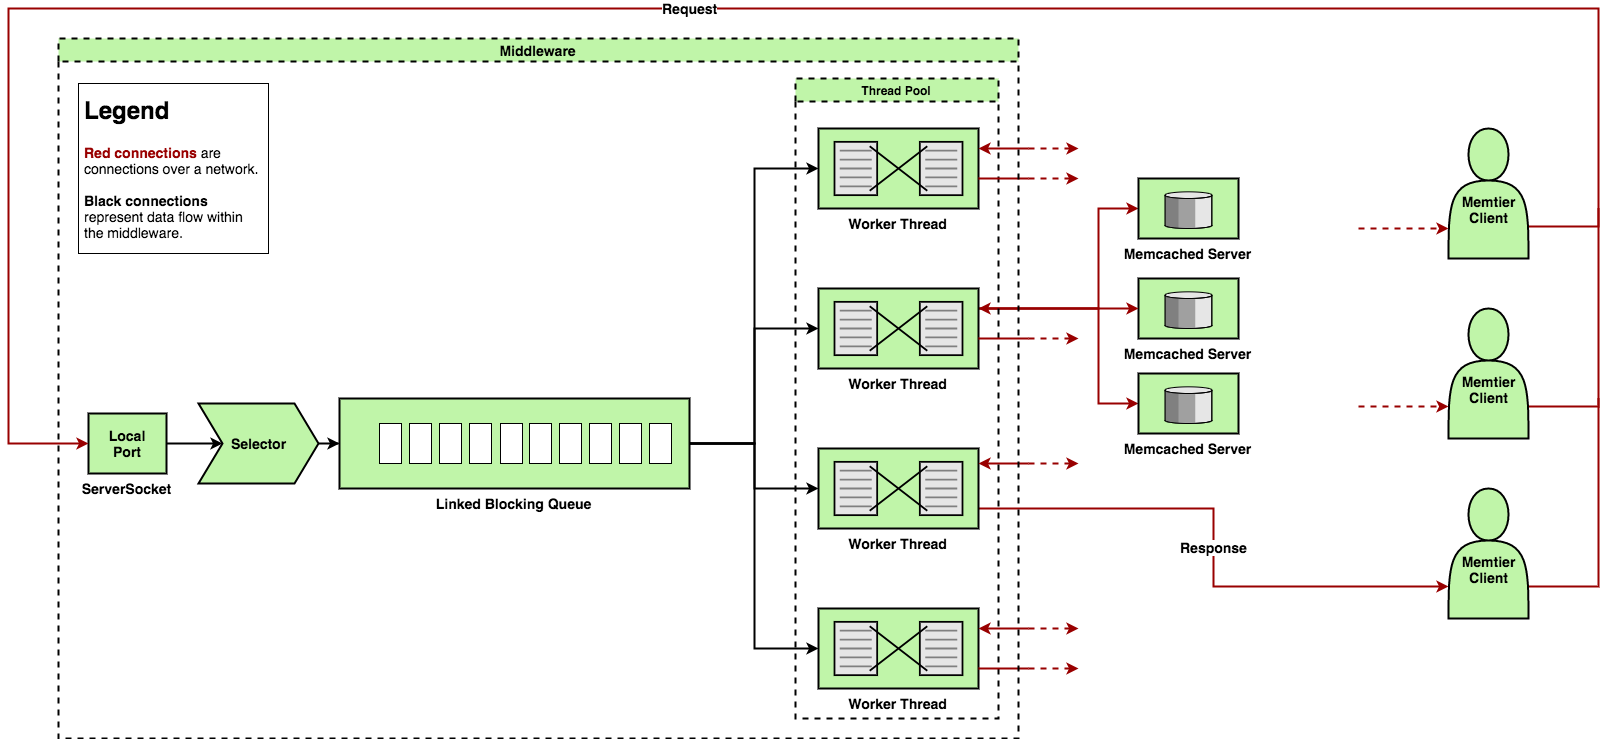
\includegraphics[width=\textwidth]{processing/graphics/system_overview.png}
    \caption{System Overview}
    \label{png::system_overview}
\end{figure}

As can be seen in figure \ref{png::system_overview}, a selector is attacked to the server socket in order to accept connections from clients. The key attached to the client connection is then passed with the request such that the workers can communicate the response back to the clients. The reason for the selector is to allow client connections to remain open until explicitly closed by the client. Hence the role of the selector is also to allow new connections and to add them to its internal register of client connections. Once in the internal register (the connection is accepted), the client can send a request which will be read by the net-thread and added to the queue with a reference to the client key. The worker threads then get requests off the queue and process them one by one. The workers first parse the request to get the command type. If the command is invalid, an error message is immediately sent back to the client associated with this request. Otherwise, the worker then communicates with the Memcached server(s) in order to store or retrieve data. The servers' response(s) are then parsed again to check for errors and statistics, and a response, potentially merged, is sent to the client.

\subsection{Selector}
The selector serves as a register for connected clients. It is used as passing a socket channel in the queue as part of the request forces the connection to be closed at completion of the request. Hence the selector accepts connections from clients and registers all connected clients. The selector then listens to the registered clients for messages sent to the server socket it is connected to and generates ``read events'' for each client sending messages to the socket. Simultaneously, the net-thread permanently checks for read events generated by the selector and reads data from the client associated with the event to a buffer. This buffer is then added as a request to the queue. Note that the selector key and a timestamp are added to the buffer to form a complete request on the queue. Moreover, note that the use of a selector forces to use non-blocking IO on the client side. However, this is not a problem since any read event guarantees that data can be read from the socket, hence avoiding the use of reading loops.

\subsection{Worker Threads}
A thread pool executor of fixed size is used to organise the worker threads. This has the advantage that it reduces thread environment switching if there is not need for an extra thread to be used. This could be the case when the connection to the Memcached servers are extremely fast. In such a case, the executor will not use more threads than than are available from the hardware as reusing the same thread to process the next request does not involve any overhead compared to switching to another thread to perform the same work. However, as soon as server service times increase, the thread pool allows to perform work on some thread while another is idle awaiting a response from Memcached. Moreover, the thread pool executor has the advantage that if some thread crashed during the execution of the middleware, it will automatically be relaunched. Hence it should in theory provide more stability to the system.

The worker threads perform close to the entirety of the work within the middleware. The reason these workers perform the most work is that the work can be performed concurrently and, ideally, it is performed in parallel. In the initial design, even the reading of the socket was performed by the workers to avoid creating a buffer (containing the message sent from the client) for each request. However, this lead to request duplication as the read event was active as long as nothing was read from the socket, hence repeatedly adding requests to the queue if the initial request had not already been read. This was easily caused by even non-significant queue times. Therefore the design was changed, at the cost of creating a byte buffer for each request.

When launching a thread, two buffers are created. One is used for temporary data while the other contains the response from Memcached to be sent back to clients. Note that all buffers used in the middleware are of size 16384 bytes as this allows for 10 keys of size 250 bytes and 10 values of 1024 bytes (and some margin) to be stored in the buffer. The temporary data buffer is mostly used to interpret individual responses from the Memcached servers and its data is then added to the buffer containing the aggregate data for the client. Creating only two buffers for each worker has the goal to reduce dead times created by the garbage collector. Exactly how individual request types are handled by the middleware and how the buffers are utilised is explained in a later section.

Each worker is connected to all backend Memcached servers at all times. These channels are blocking to ensure that the worker awaits a response from the servers when reading from a channel. Should a worker crash, the thread pool executor will rebuild a thread to replace it and the connections to the servers should be reestablished. However, note that such a situation never occurred during testing.

\subsection{Requests}
All requests are built from the following:
\begin{itemize}
    \item A buffer containing the data sent from the client. This is known when the request object is created.
    \item A selection key that refers to the client who sent the request. This is used to recover the channel to said client in order to sent him the response. Note this has nothing to do with the Memcached key used to refer to the data stored on the backend servers.
    \item A type which can be either:
    \begin{enumerate}
        \item GET: a simple get request with a single key.
        \item SET: a simple set request with one key and the data to be set as the value for that key.
        \item MULTIGET: a get request with more than one key.
        \item INVALID: a request that does not conform to the protocol defining the format of the three commands above.
    \end{enumerate}
    This is not known when the request is created and will only be known once a worker parses the request.
    \item A boolean identifying the request as a hit. Note that the notion of hit is different for each type of request. In the case of a get, it simply identifies whether a value was returned by the Memcached servers. In the case of a set, this represents whether a server responded with something different to \mintinline{java}{STORED}. In the cases of multiget and invalid request, this boolean does not have any meaning. Multiget hits are handled directly as the responses from Memcached are parsed.
    \item Several timestamps:
    \begin{enumerate}
        \item The time the request is created. This is (obviously) known when the request is created.
        \item The time the request is dequeued. The worker updates this timestamp as soon as the request is taken from the queue.
        \item The time the request was transmitted to the servers. This timestamp is taken just before any messages are sent to Memcached.
        \item The time Memcached answered. This is taken once \textit{all} Memcached servers that were contacted for this request have answered.
        \item The time the request was completed. This is the timestamp taken when the complete response was sent back to the client.
    \end{enumerate}
\end{itemize}

All requests are parsed only at the worker level, hence the majority of the fields defined above are only known once the request is being processed by some worker.

When parsing a request, the first aspect that is checked is whether the request terminates with \mintinline{java}{"\r\n"}. Then the command is parsed up to the first occurrence of \mintinline{java}{"\r\n"}. The set of bytes preceding these two characters is converted to a string and the first word in said string is compared to known command words (i.e. \mintinline{java}{get} or \mintinline{java}{set}). Once it is established which type the command is, the rest of the command is checked for correctness. In the case of \mintinline{java}{get}, the number of arguments is checked in order to determine whether the command should be treated as a \mintinline{java}{multiget}. In the case of a \mintinline{java}{set}, it is checked if the data block attacked to the request is of the length specified in the command. If any of these tests fail, the command is flagged as invalid and an error string is sent back to the client. In this case there is no communication with the backend Memcached servers as the request does not conform to the protocol.

\subsubsection{Sets}
Once a command has been dequeued, parsed, and established as type \mintinline{java}{set}, all worker buffers are cleared and the original request buffer is transmitted to all backend servers. The worker thread then awaits responses from the servers in the same order as he sent out the request. As we use blocking input/output on the server side, the same order is chosen as the first contacted server is likely the first to respond. Note however that if the connection to the first Memcached server is significantly slower than other connections, this will result in inefficient time utilisation as the middleware will wait for this response first, even though the responses from other servers might already be available. Every response is then checked and if anything other than \mintinline{java}{"STORED\r\n"} is returned from any server, that response is returned to the client and the \mintinline{java}{set} is flagged as a miss. The rest of the servers' responses are read in order to make sure all communication channels are cleared for the next request.
\begin{figure}[h]
    \centering
    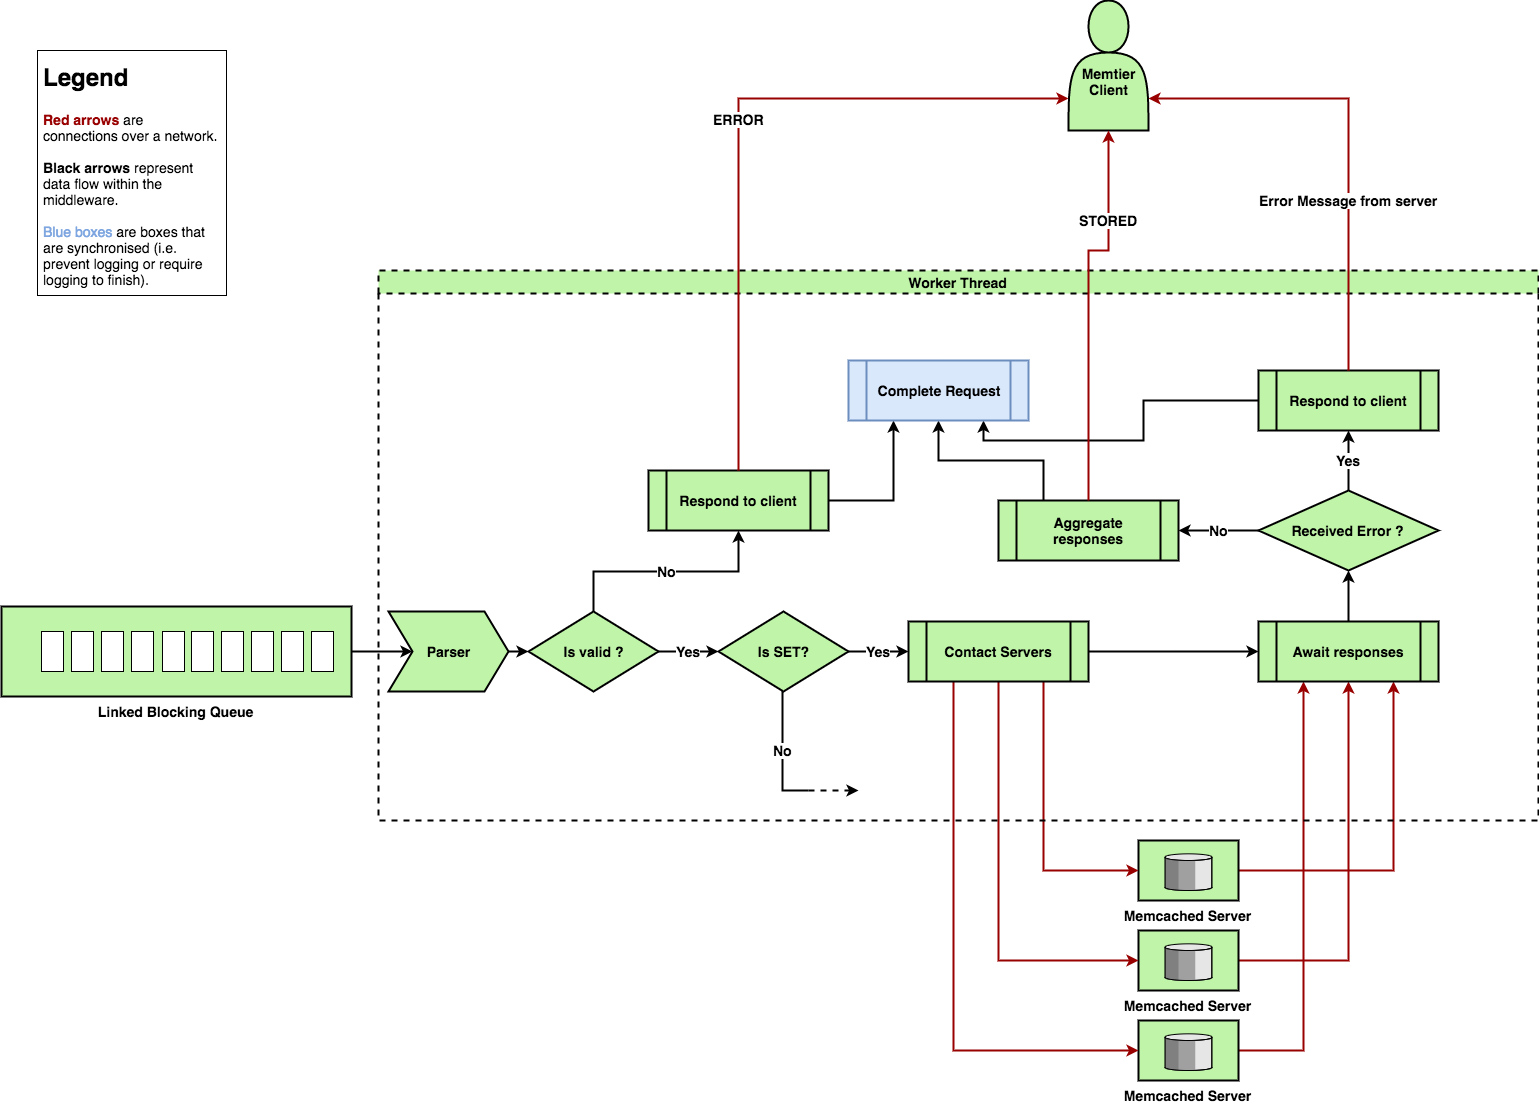
\includegraphics[width=\textwidth]{processing/graphics/sets_handling.png}
    \caption{Handling of \mintinline{java}{SET} requests}
    \label{png::sets_handling}
\end{figure}
In the case of a hit (i.e. all servers responded \mintinline{java}{"STORED\r\n"}), this is relayed to the client and the request is completed. Request completion will be described under logging and thread synchronisation below.

Note that that during the time the request is handled, the appropriate timestamps are updated for the request.

\subsubsection{Gets and Non-Sharded Multigets}
As these requests are not sent to all Memcached servers, load balancing is in order. To perform load balancing, a server is chosen by simply taking the least recently used server across all workers. Of course, this can be suboptimal if the least recently used server is still working on a large request and other servers have already freed after handling smaller requests. However, due to relatively strong variations in the network latencies, it is very difficult to predict the time needed for a server to process a request.

\begin{figure}[h]
    \centering
    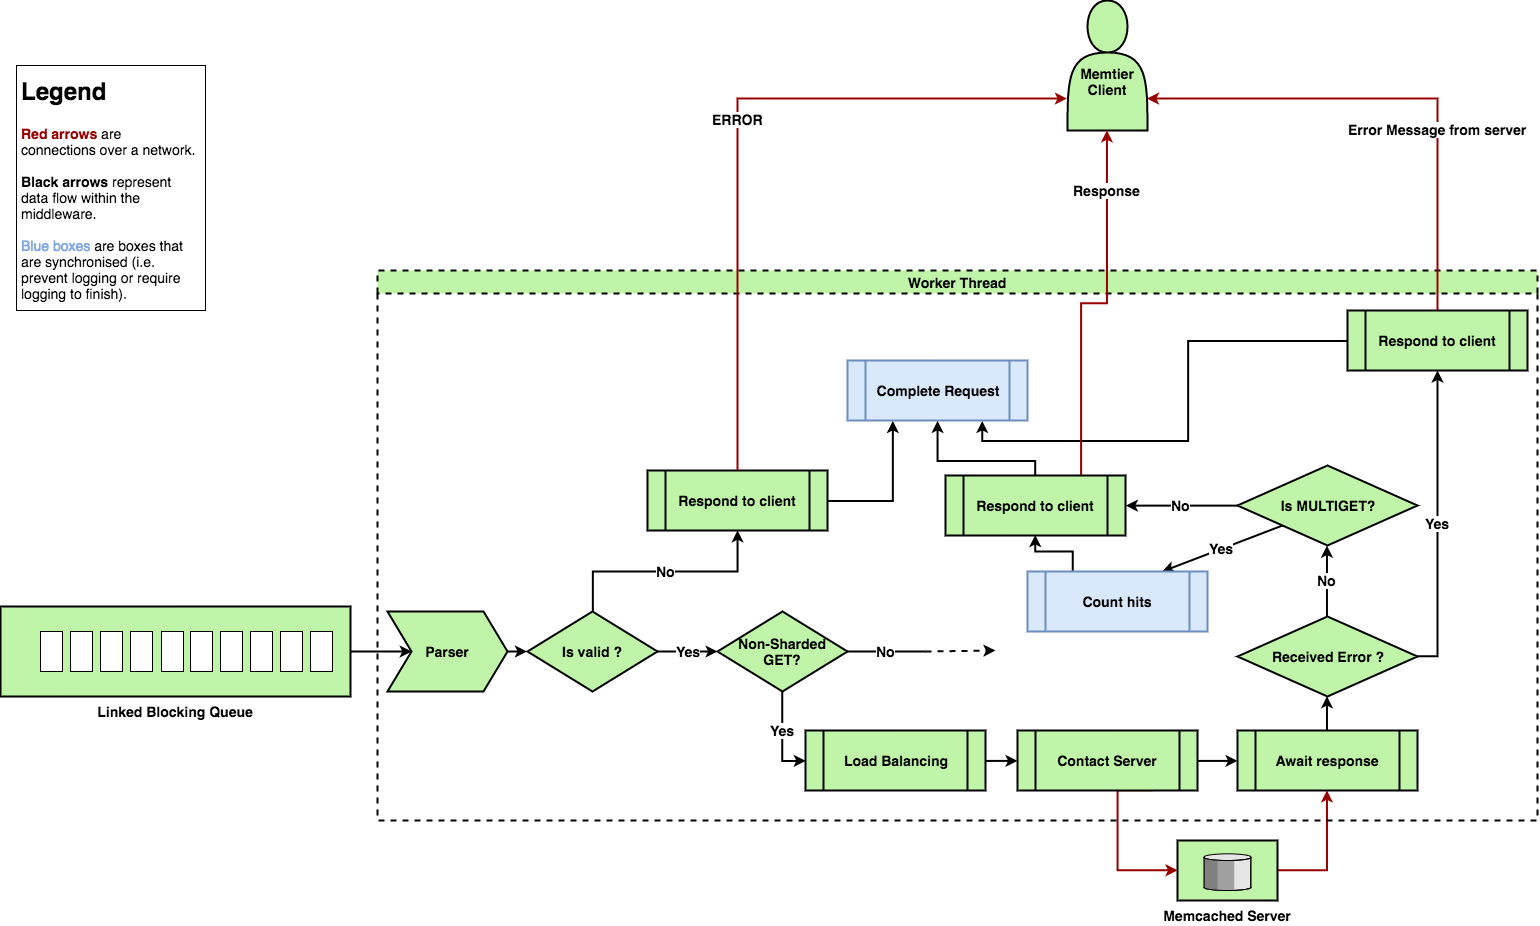
\includegraphics[width=\textwidth]{processing/graphics/gets_handling.png}
    \caption{Handling of \mintinline{java}{GET} and non-sharded \mintinline{java}{MULTIGET} requests}
    \label{png::gets_handling}
\end{figure}

The request, as it was received by the client, is then sent to the selected server. The worker awaits a answer and continuously reads from the channel until the response either ends with \mintinline{java}{"ERROR\r\n"} or matches an error (anything ending with \mintinline{java}{"ERROR\r\n"}, i.e. also \mintinline{java}{"SERVER_ERROR\r\n"} or \mintinline{java}{"CLIENT_ERROR\r\n"}). Note that this does not create a hot loop as the channel reading is blocking.

If the request is of type multiget, the worker checks how many values were included in the response compared to the number of values requested in the command. This then determined the number of hits and misses of the request.

For a get, the response is compared to \mintinline{java}{"END\r\n"} and checked if it ends with \mintinline{java}{"ERROR\r\n"}. If neither is the case, the request is flagged as a hit.

Both for \mintinline{java}{multigets} and single \mintinline{java}{get}, the response is then relayed to the client and the request completed.


\subsubsection{Sharded Multigets}
In the case of a sharded multigets, the \mintinline{java}{readSharded(request, response_buffer, temp_buffer)} function is called. This function completely takes care of the handling of such requests with the exception of request completion. Sharded requests are handled in two ways (graphically shown in figure \ref{png::multigets_handling}):
\begin{enumerate}
    \item If the number of requested values is less than the number of available Memcached servers, load balancing is performed and a single \mintinline{java}{get} is sent to a server. Again, the servers responses are interpreted in the same order as the servers were contacted. If an error is received from any server, \mintinline{java}{"ERROR\r\n"} is relayed to the client and the server channels are cleared for the next request. Otherwise individual responses are read into the temporary buffer, \mintinline{java}{"END\r\n"} is removed from the end of the buffer and the entire buffer is appended to the response buffer.
    \item If the number of request values is larger than the number of available Memcached servers, no load balancing is required as all servers will need to be contacted anyways. The processing is then performed as above.
\end{enumerate}
\begin{figure}[h]
    \centering
    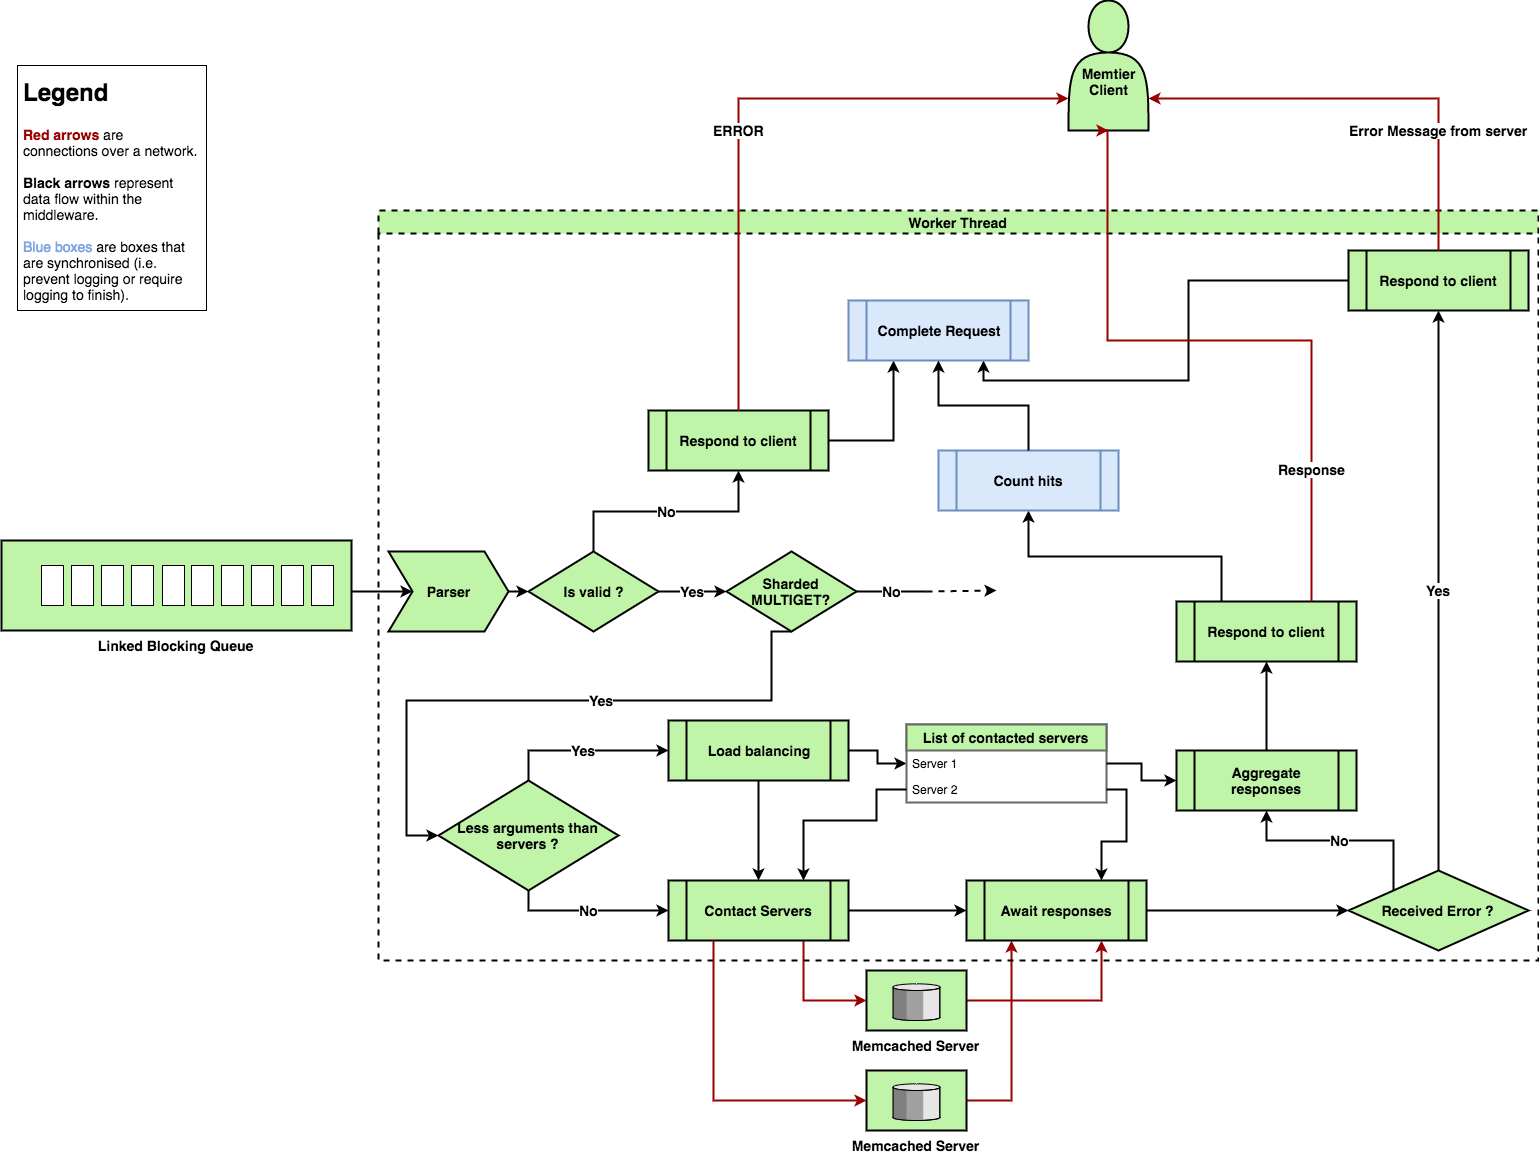
\includegraphics[width=\textwidth]{processing/graphics/multigets_handling.png}
    \caption{Handling of sharded \mintinline{java}{MULTIGET} requests}
    \label{png::multigets_handling}
\end{figure}
When all Memcached servers have answered, \mintinline{java}{"END\r\n"} is added to the response buffer and the response is relayed to the client unless an error occurred in one of the servers. The response buffer is then converted into a string to check the number of hits. Note that this is performed irrespective of a server responding \mintinline{java}{"ERROR\r\n"}.


\subsection{Logging, Request Completion and Thread Synchronisation}
All statistical data relating to a request is stored within the request itself. Hence the reserved fields for timestamps, type and hit flags. When a request is completed, the \mintinline{java}{complete(request)} private method of that worker object is called. This method is then computes the required statistics and stores them internally in the corresponding worker object. Hence note that up until the completion of the request, no internal data of the worker was touched with the exception of \mintinline{java}{multigets} hit counting.

Every part of the workers that accessed internal statistics data is synchronised with respect to the worker object. Hence both the \mintinline{java}{complete(request)} and the \mintinline{java}{multiget} hit counting are synchronised. This ensures memory data consistency when accessing the internal statistical data for logging. Hence all data should be consistent and no request should only partially logged unless the logger kicks in between two boxes in figures \ref{png::gets_handling} and \ref{png::multigets_handling}. This can only happen during the handling of multigets and creates hits to be registered even though the request is incomplete. This is very unlikely to happen as close to no work is performed between any two blue boxes. Moreover, note that this does not affect any final statistics.

The logging is performed by a static function:
\begin{minted}{java}
    public static String getRecord(ArrayList<Worker> workers, int queueLength);
\end{minted}
(of the worker class) that, when accessing the internal data of a worker in its argument list, locks that worker, hence preventing it from modifying its internal statistical data. This is done in order to get consistent interval information when logging. \\
Every second, the \mintinline{java}{getRecord()} function is called on all workers and gathers their statistical data to output what has happened in the last second. Note that this does not prevent the worker from performing work until it reaches either request completion or a multiget hit count update. Due to the fact that data gathering is relatively fast compared to the overall time needed to process a request and the server time, this usually does not affect performance. Moreover, note that not all workers are blocked but only the one currently being accessed. This can create slightly offset data when the middleware is launched with a large number of workers as the last few workers might complete some requests while the data from the first worker is being read. However, this only affects the time interval, not the overall data, because the logger only gathers data from since \mintinline{java}{getRecord()} was called \textit{on that worker}. Hence, even if the last worker completes more requests while the data from the first worker is being collected, these completed requests will not be considered the next time \mintinline{java}{getRecord()} is called on that worker.

Furthermore, \mintinline{java}{getRecord()} also takes care of clearing any histogram information stored in workers when running for the first time. This is to ensure that histogram data does not include requests completed during warm up time. The warm up time is set to ten seconds, therefore \mintinline{java}{getRecord()} is called ten seconds after the launch of the middleware and then again every second after that.

The analysis data is logged both to console and to an \mintinline{shell}{analysis.log} file in the home directory. Note that the logs in the log file additionally contain timestamps. Moreover, the middleware logs system information such as interruptions, errors settings up sockets, connection request, etc. to \mintinline{shell}{system_report.log} also in the home directory.

On top of that, when the \mintinline{java}{ShutdownHook} is triggered, statistics for individual workers is gathered and the histogram is printed. The statistic for individual workers include queue time, processing time, server time, total count, hits per second and misses per second for each request type. The final statistics layout is very similar to the one provided my memtier.


\subsection{Overall Experimental Design}
All repetitions taken are at least 90 seconds long. The ten first seconds are evicted (warm up time) and the 80 next measurements are taken as the data. For client and server data, only the first eight seconds are evicted as the automation scripts allow two seconds for the middleware to boot properly before launching the clients. Note that due to \mintinline{java}{ssh} network latencies, the 80 second windows of measurements might not perfectly coincide between clients, middleware, and servers, but this should be insignificant compared to the overall length of a repetition.




\newpage

\section{Baseline without Middleware (75 pts)}

In this experiments you study the performance characteristics of the memtier clients and memcached servers.

\subsection{One Server}

Both, for a read-only and write-only workload plot the throughput and the response time as a function of NumClients. All clients are connected to a single memcached instance.

Use 3 load generating VMs, with one memtier (CT=2) each, and vary the number of virtual clients (VC) per memtier thread between 1 and 32. Show how the behavior of the server changes as we add more clients.

\begin{center}
	\scriptsize{
		\begin{tabular}{|l|c|}
			\hline Number of servers                & 1                        \\
			\hline Number of client machines        & 3                        \\
			\hline Instances of memtier per machine & 1                        \\
			\hline Threads per memtier instance     & 2                        \\
			\hline Virtual clients per thread       & [1..32]                  \\
			\hline Workload                         & Write-only and Read-only \\
			\hline Multi-Get behavior               & N/A                      \\
			\hline Multi-Get size                   & N/A                      \\
			\hline Number of middlewares            & N/A                      \\
			\hline Worker threads per middleware    & N/A                      \\
			\hline Repetitions                      & 3 or more                \\
			\hline
		\end{tabular}
	}
\end{center}

\subsubsection{Explanation}

Describe in which phase the memcached servers are under-saturated, saturated, or over-saturated. Describe how throughput and response time correlate. Explain what further conclusions can be drawn from the experiment.


\subsection{Two Servers}

For a read-only and write-only workload plot throughput and response time as a function of NumClients. The clients are connected to two memcached instances.

Use 1 load generating VM, with one memtier (CT=1) connected to each memcached instance (two memcache instances in total), and vary the number of virtual clients (VC) per memtier thread between 1 and 32. Show how the behavior of the server changes and explain what conclusions we can draw from this experiment.

\begin{center}
	\scriptsize{
		\begin{tabular}{|l|c|}
			\hline Number of servers                & 2                        \\
			\hline Number of client machines        & 1                        \\
			\hline Instances of memtier per machine & 2                        \\
			\hline Threads per memtier instance     & 1                        \\
			\hline Virtual clients per thread       & [1..32]                  \\
			\hline Workload                         & Write-only and Read-only \\
			\hline Multi-Get behavior               & N/A                      \\
			\hline Multi-Get size                   & N/A                      \\
			\hline Number of middlewares            & N/A                      \\
			\hline Worker threads per middleware    & N/A                      \\
			\hline Repetitions                      & 3 or more (at least 1 minute each)                \\
			\hline
		\end{tabular}
	}
\end{center}

\subsubsection{Explanation}

Describe how this experiment compares to the previous section. Which results are the same and which ones differ? Explain what further conclusions can be drawn from the experiment.


\subsection{Summary}

Based on the experiments above, fill out the following table:

\begin{center}
	{Maximum throughput of different VMs.}
	\begin{tabular}{|l|p{2cm}|p{2cm}|p{4cm}|}
		\hline                        & Read-only workload & Write-only workload & Configuration gives max. throughput \\
		\hline One memcached server   &                    &                     &                                     \\
		\hline One load generating VM &                    &                     &                                     \\
		\hline
	\end{tabular}
\end{center}


Write at least two paragraphs about how both results relate. Describe what is the bottleneck of this setup is. If the maximum throughput for both experiments is the same, explain why. If it is not the case, explain why not. Write down key take-away messages about the behaviour of the memtier clients and the memcached servers.

\section{Baseline with Middleware (90 pts)}

In this set of experiments, you will have to use 1 load generator VM and 1 memcached server, measuring how the throughput of the system changes when increasing the number of clients. Scaling virtual clients inside memtier has to be done as explained in the previous sections. Plot both throughput and response time as measured on the middleware.

\subsection{One Middleware}

Connect one load generator machine (one instance of memtier with CT=2) to a single middleware and use 1 memcached server. Run a read-only and a write-only workload with increasing number of clients (between 2 and 64) and measure response time \emph{both at the client and at the middleware}, and plot the throughput and response time measured in the middleware.

Repeat this experiment for different number of worker threads inside the middleware: 8, 16, 32, 64.

\begin{center}
	\scriptsize{
		\begin{tabular}{|l|c|}
			\hline Number of servers                & 1                        \\
			\hline Number of client machines        & 1                        \\
			\hline Instances of memtier per machine & 1                        \\
			\hline Threads per memtier instance     & 2                        \\
			\hline Virtual clients per thread       & [1..32]                  \\
			\hline Workload                         & Write-only and Read-only \\
			\hline Multi-Get behavior               & N/A                      \\
			\hline Multi-Get size                   & N/A                      \\
			\hline Number of middlewares            & 1                        \\
			\hline Worker threads per middleware    & [8..64]                  \\
			\hline Repetitions                      & 3 or more (at least 1 minute each)                \\
			\hline
		\end{tabular}
	}
\end{center}

\subsubsection{Explanation}

Provide a detailed analysis of the results (e.g., bottleneck analysis, component utilizations, average queue lengths, system saturation). Add any additional figures and experiments that help you illustrate your point and support your claims.

\subsection{Two Middlewares}

Connect one load generator machine (two instances of memtier with CT=1) to two middlewares and use 1 memcached server. Run a read-only and a write-only workload with increasing number of clients (between 2 and 64) and measure response time \emph{both at the client and at the middleware}, and plot the throughput and response time as measured in the middleware.

Repeat this experiment for different number of worker threads inside the middleware: 8, 16, 32, 64.

If in your experiment the middleware is not the bottleneck, repeat the experiment that reaches the highest throughput but using two load generator VMs (each with 2x memtier CT=1) instead of one. Otherwise, explain how you know that the middlewares are the limiting factor in terms of throughput.

\begin{center}
	\scriptsize{
		\begin{tabular}{|l|c|}
			\hline Number of servers                & 1                        \\
			\hline Number of client machines        & 1                        \\
			\hline Instances of memtier per machine & 2                        \\
			\hline Threads per memtier instance     & 1                        \\
			\hline Virtual clients per thread       & [1..32]                  \\
			\hline Workload                         & Write-only and Read-only \\
			\hline Multi-Get behavior               & N/A                      \\
			\hline Multi-Get size                   & N/A                      \\
			\hline Number of middlewares            & 2                        \\
			\hline Worker threads per middleware    & [8..64]                  \\
			\hline Repetitions                      & 3 or more (at least 1 minute each)                \\
			\hline
		\end{tabular}
	}
\end{center}

\subsubsection{Explanation}

Provide a detailed analysis of the results (e.g., bottleneck analysis, component utilizations, average queue lengths, system saturation). Add any additional figures and experiments that help you illustrate your point and support your claims.

\subsection{Summary}

Based on the experiments above, fill out the following table. For both of them use the numbers from a single experiment to fill out all lines. Miss rate represents the percentage of GET requests that return no data. Time in the queue refers to the time spent in the queue between the net-thread and the worker threads.


\begin{center}
	{Maximum throughput for one middleware.}
	\begin{tabular}{|l|p{2cm}|p{2cm}|p{2cm}|p{2cm}|}
		\hline                                & Throughput & Response time & Average time in queue & Miss rate \\
		\hline Reads: Measured on middleware  &            &               &                       &           \\
		\hline Reads: Measured on clients     &            &               & n/a                   &           \\
		\hline Writes: Measured on middleware &            &               &                       & n/a       \\
		\hline Writes: Measured on clients    &            &               & n/a                   & n/a       \\
		\hline
	\end{tabular}
\end{center}

\begin{center}
	{Maximum throughput for two middlewares.}
	\begin{tabular}{|l|p{2cm}|p{2cm}|p{2cm}|p{2cm}|}
		\hline                                & Throughput & Response time & Average time in queue & Miss rate \\
		\hline Reads: Measured on middleware  &            &               &                       &           \\
		\hline Reads: Measured on clients     &            &               & n/a                   &           \\
		\hline Writes: Measured on middleware &            &               &                       & n/a       \\
		\hline Writes: Measured on clients    &            &               & n/a                   & n/a       \\
		\hline
	\end{tabular}
\end{center}

Based on the data provided in these tables, write at least two paragraphs summarizing your findings about the performance of the middleware in the baseline experiments.

\section{Throughput for Writes (90 pts)}

\subsection{Full System}

Connect three load generating VMs to two middlewares and three memchached servers. Run a write-only experiment.
You need to plot throughput and response time measured on the middleware as a function of number of clients. The measurements have to be performed for 8, 16, 32 and 64 worker threads inside each middleware.

\begin{center}
	\scriptsize{
		\begin{tabular}{|l|c|}
			\hline Number of servers                & 3          \\
			\hline Number of client machines        & 3          \\
			\hline Instances of memtier per machine & 2          \\
			\hline Threads per memtier instance     & 1          \\
			\hline Virtual clients per thread       & [1..32]    \\
			\hline Workload                         & Write-only \\
			\hline Multi-Get behavior               & N/A        \\
			\hline Multi-Get size                   & N/A        \\
			\hline Number of middlewares            & 2          \\
			\hline Worker threads per middleware    & [8..64]    \\
			\hline Repetitions                      & 3 or more (at least 1 minute each)  \\
			\hline
		\end{tabular}
	}
\end{center}

\subsubsection{Explanation}

Provide a detailed analysis of the results (e.g., bottleneck analysis, component utilizations, average queue lengths, system saturation). Add any additional figures and experiments that help you illustrate your point and support your claims.

\subsection{Summary}

Based on the experiments above, fill out the following table with the data corresponding to the maximum throughput point for all four worker-thread scenarios.

\begin{center}
	{Maximum throughput for the full system}
	\begin{tabular}{|l|p{1.5cm}|p{1.5cm}|p{1.5cm}|p{1.5cm}|}
		\hline                                            & WT=8 & WT=16 & WT=32 & WT=64 \\
		\hline Throughput (Middleware)                    &      &       &       &       \\
		\hline Throughput (Derived from MW response time) &      &       &       &       \\
		\hline Throughput (Client)                        &      &       &       &       \\
		\hline Average time in queue                      &      &       &       &       \\
		\hline Average length of queue                    &      &       &       &       \\
		\hline Average time waiting for memcached         &      &       &       &       \\
		\hline
	\end{tabular}
\end{center}

Based on the data provided in these tables, draw conclusions on the state of your system for a variable number of worker threads.

\section{Gets and Multi-gets (90 pts)}

For this set of experiments you will use three load generating machines, two middlewares and three memcached servers. Each memtier instance should have 2 virtual clients in total and the number of middleware worker threads is 64, or the one that provides the highest throughput in your system (whichever number of threads is smaller).

For multi-GET workloads, memtier will generate a mixture of SETs, GETs, and multi-GETs. Memtier only allows to specify the maximum number of keys in a multi-GET request. Therefore, be aware that requests can also contain fewer keys than the provided value. It is recommended to record the average size of the multi-GETs. You will have to measure response time on the client as a function of multi-get size, with and without sharding on the middlewares.

\subsection{Sharded Case}

Run multi-gets with 1, 3, 6 and 9 keys (memtier configuration) with sharding enabled (multi-gets are broken up into smaller multi-gets and spread across servers). Plot average response time as measured on the client, as well as the 25th, 50th, 75th, 90th and 99th percentiles.

\begin{center}
	\scriptsize{
		\begin{tabular}{|l|c|}
			\hline Number of servers                & 3                       \\
			\hline Number of client machines        & 3                       \\
			\hline Instances of memtier per machine & 2                       \\
			\hline Threads per memtier instance     & 1                       \\
			\hline Virtual clients per thread       & 2     		            \\
			\hline Workload                         & memtier-default             \\
			\hline Multi-Get behavior               & Sharded                 \\
			\hline Multi-Get size                   & [1..9]                  \\
			\hline Number of middlewares            & 2                       \\
			\hline Worker threads per middleware    & max. throughput config. \\
			\hline Repetitions                      & 3 or more (at least 1 minute each)               \\
			\hline
		\end{tabular}
	}
\end{center}

\subsubsection{Explanation}

Provide a detailed analysis of the results (e.g., bottleneck analysis, component utilizations, average queue lengths, system saturation). Add any additional figures and experiments that help you illustrate your point and support your claims.

\subsection{Non-sharded Case}

Run multi-gets with 1, 3, 6 and 9 keys (memtier configuration) with sharding disabled. Plot average response time as measured on the client, as well as the 25th, 50th, 75th, 90th and 99th percentiles.

\begin{center}
	\scriptsize{
		\begin{tabular}{|l|c|}
			\hline Number of servers                & 3                       \\
			\hline Number of client machines        & 3                       \\
			\hline Instances of memtier per machine & 2                       \\
			\hline Threads per memtier instance     & 1                       \\
			\hline Virtual clients per thread       & 2                		 \\
			\hline Workload                         & memtier-default             \\
			\hline Multi-Get behavior               & Non-Sharded             \\
			\hline Multi-Get size                   & [1..9]                  \\
			\hline Number of middlewares            & 2                       \\
			\hline Worker threads per middleware    & max. throughput config. \\
			\hline Repetitions                      & 3 or more (at least 1 minute each)               \\
			\hline
		\end{tabular}
	}
\end{center}

\subsubsection{Explanation}

Provide a detailed analysis of the results (e.g., bottleneck analysis, component utilizations, average queue lengths, system saturation). Add any additional figures and experiments that help you illustrate your point and support your claims.

\subsection{Histogram}

For the case with 6 keys inside the multi-get, display four histograms representing the sharded and non-sharded response time distribution, both as measured on the client, and inside the middleware. Choose the bucket size in the same way for all four, and such that there are at least 10 buckets on each of the graphs.

\subsection{Summary}

Provide a detailed comparison of the sharded and non-shareded modes. For which multi-GET size is sharding the preferred option? Provide a detailed analysis of your system. Add any additional figures and experiments that help you illustrate your point and support your claims.

\section{2K Analysis (90 pts)}

For 3 client machines (with 64 total virtual clients per client VM) measure the throughput and response time of your system in a 2k experiment with repetitions. All GET operations have a single key. Investigate the following parameters:

\begin{itemize}

	\item Memcached servers: 2 and 3
	\item Middlewares: 1 and 2
	\item Worker threads per MW: 8 and 32

\end{itemize}

Repeat the experiment for (a)~a write-only, (b)~a read-only, and (c)~a 50-50-read-write workload.
For each of the three workloads, what is the impact of these parameters on throughput, respectively response time?

\begin{center}
	\scriptsize{
		\begin{tabular}{|l|c|}
			\hline Number of servers                & 2 and 3                                     \\
			\hline Number of client machines        & 3                                           \\
			\hline Instances of memtier per machine & 2                                           \\
			\hline Threads per memtier instance     & 1                                           \\
			\hline Virtual clients per thread       & 32                                     \\
			\hline Workload                         & Write-only, Read-only, and 50-50-read-write \\
			\hline Multi-Get behavior               & N/A                                         \\
			\hline Multi-Get size                   & N/A                                         \\
			\hline Number of middlewares            & 1 and 2                                     \\
			\hline Worker threads per middleware    & 8 and 32                                    \\
			\hline Repetitions                      & 3 or more (at least 1 minute each)                                   \\
			\hline
		\end{tabular}
	}
\end{center}

\section{Queuing Model (90 pts)}

Note that for queuing models it is enough to use the experimental results from the previous sections. It is, however, possible that the numbers you need are not only the ones in the figures we asked for, but also the internal measurements that you have obtained through instrumentation of your middleware.

\subsection{M/M/1}

Build queuing model based on Section 4 (write-only throughput) for each worker-thread configuration of the middleware. Use one M/M/1 queue to model your entire system. Motivate your choice of input parameters to the model. Explain for which experiments the predictions of the model match and for which they do not.

\subsection{M/M/m}

Build an M/M/m model based on Section 4, where each middleware worker thread is represented as one service.  Motivate your choice of input parameters to the model. Explain for which experiments the predictions of the model match and for which they do not.

\subsection{Network of Queues}

Based on Section 2, build a network of queues which simulates your system. Motivate the design of your network of queues and relate it wherever possible to a component of your system. Motivate your choice of input parameters for the different queues inside the network. Perform a detailed analysis of the utilization of each component and clearly state what the bottleneck of your system is. Explain for which experiments the predictions of the model match and for which they do not.

\end{document}
